\section{AutoFAME}
\subsection{FAME Introduction}
FAME, or FPGA Architecture Model Execution is a system for efficiently emulating digital circuits on a FPGA introduced in the \textit{A Case for FAME: FPGA Architecture Model Execution paper} \cite{FAME:2010}. The paper introduces a system in which the concept of the emulated digital circuit, hence known as the target machine, is separated from the concept of the digital circuit that does the emulation of the target machine, hence known as the host machine. By extension, in FAME, the concept of time passing in the target machine, hence known as target time, is separated from the concept of time passing in the host machine, hence known as host time. 

In naive FPGA emulation, the target machine and the host machine are the same digital circuit. the RTL specification of the target machine is mapped directly to an FPGA through vendor tools with no change in the logic design. Because the characteristics of a FPGA are sometimes significantly different from the characteristics of a ASIC in timing and area characteristics, it is desirable to use a modified implementation of the design to emulation on a FPGA. In an modified implementation optimized for an FPGA, the host machine maybe different from the target machine and it may take more than one or less than one host clock cycle emulate one target clock cycle.

Using FAME, large digital designs can be broken up into modules that talk to each other in a decoupled manner. The partitioned system maintains the same target time behavior as the original design even though the modules are communicating in a decoupled manner. Once the original design is partitioned into decoupled modules, modules can be individually optimzed for FPGA emulation, with no restrictions on the host time to target time relationship in each module, while preserving the same target time behavior of the whole system as the target time behavior of the original design.

The original design to be emulated is called a FAME0 level design. The original design should be viewed as a set of FAME0 level modules connected together by registers and queues. A FAME0 module naively modified to work as a module that can be inserted into the partitioned system of decoupled modules is called a FAME1 level module. Figure \ref{fig:fame-partition} shows a FAME0 design being transformed intoa FAME1 design. A module that can be inserted into the partitioned system of decoupled modules and emulates a FAME0 module in an abstract manner, such as with a split functional model/timing model implementation of the FAME0 module, is called a FAME3 level module. A single module that can be inserted into the partitioned system of decoupled modules and emulates n copies of a FAME0 module through multi-threading is called a FAME5 level module. 

\begin{figure*}
	\centering
    \resizebox{1.5\columnwidth}{!}{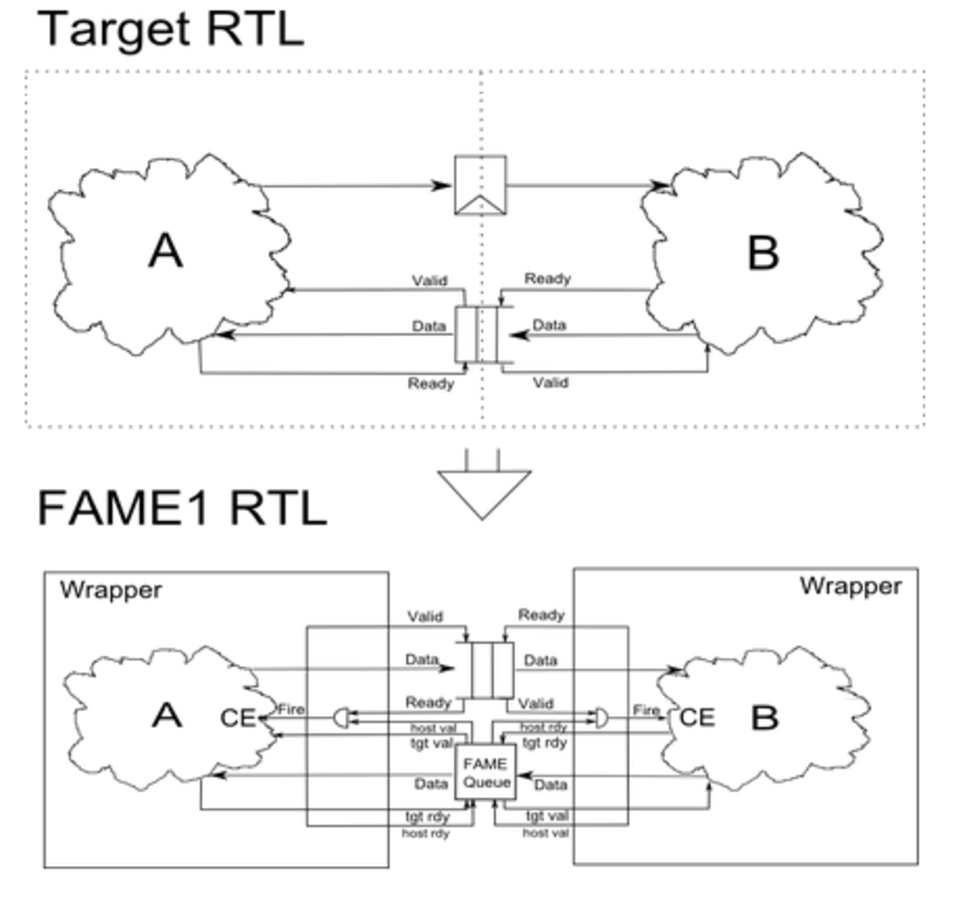
\includegraphics{figures/FAME-partition}}
    \caption{Transforming a FAME0 Design into a FAME1 Design}
	\label{fig:fame-partition}
\end{figure*}

\subsubsection{FAME Design Partitioning Details}
Target time behavior is maintained in the partitioned system in the following manner. The original design is partitioned by placing module boundaries across registers and queues in the target machine. The target machine registers are replaced by FAME Registers and the target machine queues are replaced by FAME Queues. The FAME Register is a FIFO containing tokens that represent the state of the target register at particular target clock cycles. Tokens furthur a ahead in the FIFO represent the state of the target register at earlier target clocks. The FAME Queue is a FIFO containing tokens that represent the state of the target queue at particular target clock cycles. Tokens furthur ahead in the FIFO represent the state of the target queue at earlier target clocks. Both FAME Registers and FAME Queues are initialized with one token. 

It is important to separate these tokens, which represent one target clock cycle's worth of information about the target register or target queue, from the entries in the target queues. Enqueuing/dequeuing tokens from FAME Registers/FAME Queues will be referred to as host enqueue/host dequeue and the host enqueue/dequeue operations will be performed through manipulating host ready and host valid signals. If a FAME Register/FAME Queue does not contain any tokens, it will be referred to as host empty and if a FAME Register/FAME Queue cannot accept any more tokens, it will be referred as host full. In contrast, enqueueing/dequeue entries from the target queues will be referred to as target enqueue/target dequeue and the full/empty status of the target queues will be referred to as target full/target empty.

For every advance of the target clock, each module consumes a token from its input FAME Registers/FAME Queues and outputs a token to its output FAME Registers/FAME Queues. A module may not advance its target clock if any of its inputs are host empty or if any of its outputs are host full. Since FAME Registers and FAME Queues are FIFOs of tokens, tokens are allowed to accumulate with in FAME Registers and FAME Queus. Thus, the target clock can advance in a decoupled manner while still remaining functionally the same as the original design. 

\subsubsection{AutoFAME Features}
AutoFAME is capable of creating FAME1 and FAME5 level FPGA optimized designs given a base functional datapath specified in Chisel. This is equivalent of automatically transforming a FAME0 level design into a FAME1 or FAME5 level design. The tool performs the required circuit transformations on the Chisel internal node graph and leverages Chisel's elaboration steps to output the optimzed design as either a cycle accurate C++ emulator or as a Verilog source file. 

\subsection{Input Datapath Restrictions}
\label{section:fameRestrictions}
Because the orignal design to be emulated should be split by having module boundaries placed across registers or queues, the input FAME0 module should have IO ports of the type RegIO, which consists of a single data pin and indicates that the IO port should be connected to a register in the original design, and QueueIO, which consists of a ready pin, a valid pin, and a data pin, and indicates that the IO port should be connected to a queue in the original design.

\subsection{FAME1 Transform}
Given any FAME0 module that follows the restrictions in \ref{section:fameRestrictions} and a user annotation in the Chisel source file containing the module instantiation of the input FAME0 module that a FAME0 to FAME1 transformation should be applied, AutoFAME will produce a FAME1 version of that module.

Automatically transforming a FAME0 level design into a FAME1 level design is useful because it allows the FAME0 level design to be interfaced with FAME3 or FAME5 level designs at the cost of no extra work by the designer.

\subsubsection{Transformation}
In order to make a FAME0 module work in the partitioned system of decoupled modules, its RegIOs need to be converted into FAMERegIOs, which attach a host ready and a host valid pin to the RegIO port in order to interface with the FAME Registers. Its DecoupledIOs also need to be converted into FAMEDecoupledIOs, which also attach a host ready and a host valid pin to the DecoupledIO in order to do host enqueue/dequeues.

Then every state element write enable signal is masked with a fire target clock signal. The fire target clock signal is driven low whenever any of the input FAME Registers/FAME Queues are host empty or any of the output FAME Registers/FAME Queues are host full.

Then combinational logic is generated to host dequeue the input FAME Registers/FAME Queues and enqueue the output FAME Registers/FAME Queues whenever fire target clock is high.

\subsubsection{Example Application}
Automatic FAME0 to FAME1 transformation was used to interface a FAME0 level high performance research RISC processor used by UC Berkeley's ASPIRE Lab with a FAME3 level hardware DRAM model for FPGA emulation. The hardware FAME3 level DRAM model is necessary to get accurate results for the processor in FPGA emulation because the relative DRAM to processor clock rate on a FPGA is much higher than the relative DRAM to processor clock rate on a ASIC. In order to obtain performance figures accurate to the ASIC implementation in emulation, the FAME3 hardware DRAM model is used as a intermediary between the processor and the FPGA DRAM and makes the FPGA DRAM appear slower to the processor. Additionally, the FAME3 hardware DRAM model can be adjusted to simulate a variety of DRAM configurations, which would not be possible if the processor interfaced directly with the FPGA DRAM.

\subsection{FAME5 Transform}
Given any FAME0 module that follows the restrictions in \ref{section:fameRestrictions} and a user annotation in the Chisel source file containing the module instantiation of the input FAME0 module that a FAME0 to FAME5 transformation should be applied along with a specification of how many threads there should be, AutoFAME will produce a FAME5 version of that module.

Automatically transforming a FAME0 module into a FAME5 level design is useful because it allows the designer to conserve area usage on the FPGA if the FAME0 level design is instantiated many times as the multi-threading only replicates the state elements and not the combinational logic in the FAME0 design. Additionally, the multi-threading allows external memory access latencies to be hidden.

\subsubsection{Transformation}
First, all of the IO ports and the state elements are replicated n times, where n is the user specified number of threads.

Then, like the FAME0 to FAME1 transformation, the RegIOs and Decoupled IOs the input FAME0 design are replaced with FAMERegIOs and FAMEDecoupledIOs.

Then, a IO Ready signal and a Thread Selected signal is generated by each thread. The IO Ready signal of thread m is driven high when all of the input ports associated with thread m are not host empty and all of the output ports associated with thread m are not host full. The Thread Selected signal for thread m is high when the thread select id generated by the thread scheduler equals m.

Then, a fire target clock signal is created for each thread. Thread m's fire target clock signal when thread m's IO Ready signal is high and thread m's Thread Selected Signal is high. The write enables of all the state elements associated with thread m are then masked with the fire target clock signal of thread m.


